%  !TeX  root  =  user_guide.tex

\chapter{Работа с проекциями}\label{label_projections}
\index{проекции!работа с}

% when the revision of a section has been finalized,
% comment out the following line:
% \updatedisclaimer

В QGIS реализована возможность работы с проекциями. Проекция может быть
установлена как глобально "--- её параметры будут применены к любому
векторному слою, не содержащему информации о проекции, так и отдельно для
проекта. Кроме того, существует возможность создания собственных проекций,
а также реализована поддержка перепроецирования <<на лету>> для векторных
и растровых слоёв. Все эти функции позволяют корректно отображать
одновременно несколько слоёв, находящихся в различных проекциях.

\section{Обзор поддержки проекций}\label{label_projoverview}

QGIS поддерживат порядка 2700 известных проекций. Описание каждой из них
хранится в специальной базе данных SQLite, устанавливаемой одновременно
с QGIS. Непосредственная работа с ней не предусмотрена, поскольку данная
процедура может привести к полному отказу поддержки проекций. Описание
собственных проекций хранится отдельно, в пользовательской базе данных.
За информацией об управлении собственными проекциями обратитесь к
Разделу~\ref{sec:customprojections}.

Все проекции в QGIS основаны на базе идентификаторов European Petroleum
Group (ESPG)\index{EPSG} и Institut Geographique National of France (IGNF)\index{IGNF}
и в значительной степени абстрагированы от таблицы spatial\_references в
PostGIS\index{PostGIS} версии 1.x. EPSG-коды хранятся в базе данных и
могут быть использованы для определения проекции.

Для корректной работы перепроецирования <<на лету>> слой должен содержать
информацию о проекции, в которой хранятся данные, либо она должна быть
определена самостоятельно на уровне слоя или проекта. Для слоёв PostGIS
QGIS использует идентификатор проекции, определяемый в момент создания
слоя. Для данных, хранящихся в форматах, поддерживаемых OGR, информация
о проекции должна быть представлена в соответствующем файле, структура которого
определяется форматом. В случае shape-файлов "--- это файл, содержащий описание
проекции в формате Well Known Text (WKT)\index{WKT} и имеющий то же имя,
что и shape-файл, но с расширением *.prj. Например, для файла \filename{alaska.shp}
файлом описания проекции будет \filename{alaska.prj}.

Всякий раз, когда происходит выбор новой проекции, используемые единицы
слоя автоматически изменяются, что можно увидеть, перейдя во вкладку
\tab{Общие} диалогового окна \dropmenuopttwo{mActionOptions}{Свойства
проекта}, открываемого по нажатию кнопки \mainmenuopt{Редактировать} (Gnome,
OS\,X) или \mainmenuopt{Настройки} (KDE, Windows).

\section{Выбор проекции}
\index{проекции!выбор}
\label{sec:projection-specifying}

\begin{figure}[bt]
   \centering
   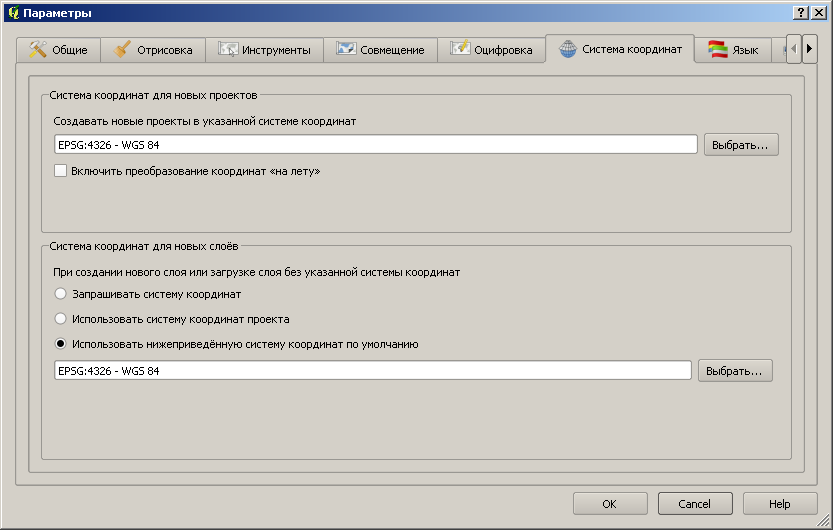
\includegraphics[clip=true, width=12cm]{crsdialog}
   \caption{Вкладка Система координат диалогового окна Параметры \wincaption}\label{fig:crsdialog}
\end{figure}

QGIS создаёт новые проекты с использованием системы координат по умолчанию.
Изначально используется система координат EPSG:4326 - WGS 84 (\texttt{proj=longlat
+ellps=WGS84 +datum=WGS84 +no\_defs}), но это поведение можно изменить
на вкладке \tab{Система координат} (см. Рисунок ~\ref{fig:crsdialog}),
вызвав из меню \mainmenuopt{Установки} \arrow \dropmenuopttwo{mActionOptions}{Параметры}
одноименный диалог.

При загрузке в проект слоёв, не содержащих информации о проекции, необходимо
иметь возможность контролировать и определять проекции таких слоёв. Проекции
могут быть установлены глобально или на уровне проекта. Для выполнения этой
операции перейдите во вкладку \tab{Система координат} окна, открываемого
через \mainmenuopt{Редактирование} \arrow \dropmenuopttwo{mActionOptions}{Параметры}
(Gnome, OSX) или \mainmenuopt{Установки} \arrow \dropmenuopttwo{mActionOptions}{Параметры}
(KDE, Windows). Смотри Рисунок~\ref{fig:crsdialog}.

На вкладке \tab{Система координат} можно выбрать один из трех режимов:
\begin{itemize}[label=--]
\item \checkbox{Запрашивать систему координат}
\item \checkbox{Использовать значение по умолчанию для данного проекта}
\item \checkbox{Использовать нижеприведённую глобальную систему координат}
\end{itemize}

Если необходимо задать проекцию для слоя, в котором информация о ней
отсутствует, то это можно сделать во вкладке \tab{Общие} окна свойств растрового
(\ref{label_generaltab}) или векторного (\ref{vectorgeneraltab}) слоя. Если
слой уже содержит информацию о проекции, то вкладка будет выглядеть как показано
на Рисунке~\ref{fig:vector_symbology}.

\begin{Tip}
\caption{\textsc{Установка системы координат из списка слоёв}} В контекстном
меню слоя есть (см. Раздел~\ref{label_legend}) присутсвует два пункта меню
для установки системы координат.
\begin{itemize}
\item \dropmenuopt{Изменить систему координат} открывает диалоговое окно
 \dialog{Выбор системы координат}. Аналогичного результата можно добиться
 нажав на кнопку \button{Система координат} на вкладке \button{Общие}
 диалогового окна \dialog{Свойства слоя}.
\item \dropmenuopt{Выбрать систему координат слоя для проекта} переопределяет
систему координат проекта так, чтобы она соответствовала системе координат
слоя
\end{itemize}
\end{Tip}

\section{Перепроецирование <<на лету>>}\label{label_projstart}

\qg поддерживает перепроецирование растровых и векторных слоёв <<на лету>>,
но по умолчанию эта возможность отключена. Для её активации необходимо
установить флажок \checkbox{Включить преобразование координат <<на лету>>}
на вкладке \tab{Система координат} диалогового окна \dropmenuopttwo{mActionProjectProperties}{Свойства
проекта}.

Существует два способа доступа к указанной вкладке:
\begin{enumerate}
\item Выберите пункт \dropmenuopttwo{mActionOptions}{Свойства проекта} меню
\mainmenuopt{Редактирование} (Gnome, OS\,X) или \mainmenuopt{Установки} (KDE,
Windows).
\item Нажмите кнопку \toolbtntwo{geographic}{Преобразование координат}, расположенную в
правом нижнем углу строки состояния.
\end{enumerate}

Также можно включить перепроецирование <<на лету>> для всех новых проектов.
Для этого необходимо установить флажок\checkbox{Включить преобразование
координат <<на лету>>} на вкладке \tab{Система координат} диалогового окна
\dialog{Параметры}.

Если имеется загруженный в проект слой и вы желаете включить перепроецирование
<<на лету>>, то откройте вкладку \tab{Система координат} диалогового окна
\dialog{Свойства проекта}, выберите проекцию для загруженного слоя и
отметьте пункт
\checkbox{Включить преобразование координат <<на лету>>}. Значок \\
\toolbtntwo{geographic}{Преобразование координат} станет активным и все
последующие загружаемые слои будут автоматически перепроецироваться в
выбранную проекцию.

Вкладка \tab{Система координат} диалогового окна \dialog{Свойства проекта}
содержит пять важных компонентов, показанных на Рисунке~\ref{fig:projections} и
описанных ниже.

\begin{figure}[ht]
   \centering
   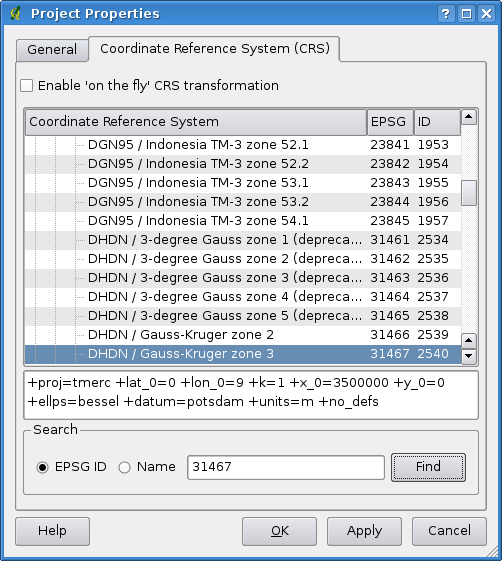
\includegraphics[clip=true, width=10cm]{projectionDialog}
   \caption{Диалоговое окно выбора проекции \wincaption}\label{fig:projections}
\end{figure}

\begin{enumerate}
\item \textbf{Включить преобразование координат <<на лету>>}\index{проекции!включение}
"--- данный пункт используется для включения или отключения преобразования
координат <<на лету>>. Если он отключен, то каждый слой отрисовывается в
соответствии с проекцией, указанной в источнике данных. Если включен, то
координаты слоя перепроецируются в проекцию карты.
\item \textbf{Система координат} "--- список проекций, поддерживаемых QGIS,
включая географические, прямоугольные и пользовательские. Для выбора проекции
выделите её имя в списке, предварительно развернув нужный узел. Текущая
проекция выделена цветом.
\item \textbf{Proj4} "--- текстовое представление проекции в формате
PROJ.4. Данный текст доступен только для чтения и используется в
качестве справочной информации.
\item \textbf{Поиск} "--- если вам известен EPSG-код, идентификатор или имя
проекции, то можно воспользоваться поиском. Введите идентификатор и нажмите
кнопку \button{Найти}. Отметьте пункт \\
\checkbox{Скрыть устарвшие системы координат}, чтобы показывать только
используемые в настоящее время проекции.
\item \textbf{Недавно использованные системы координат} "--- если имеются
определённые наиболее часто используемые в проектах проекции, то они будут
доступны в таблице, расположенной в нижней части вкладки \tab{Система координат}.
\end{enumerate}

\begin{Tip}
\caption{\textsc{Диалоговое окно Свойства проекта}}
Если открыть \dialog{Свойства проекта} из меню \mainmenuopt{Редактирование}
(Gnome, OS\,X) или \mainmenuopt{Установки} (KDE, Windows), то для доступа к
настройкам проекций нужно перейти во вкладку \tab{Система координат}. Если
же воспользоваться кнопкой
\toolbtntwo{geographic}{Преобразование координат}, то вкладка
\tab{Система координат} откроется автоматически.
\end{Tip}

\section{Определение собственной проекции}\label{sec:customprojections}
\index{проекции!пользовательские}

Если вы не нашли нужной проекции, то можно определить собственную. Для этого
выберите пункт \\
\dropmenuopttwo{mIconNew}{Ввод системы координат} меню
\mainmenuopt{Редактирование} (Gnome, OS\,X) или \mainmenuopt{Установки} (KDE,
Windows). Пользовательские проекции хранятся в пользовательской базе
данных. Помимо собственных проекций эта база содержит пространственные
закладки и прочую информацию.

\begin{figure}[ht]
   \centering
   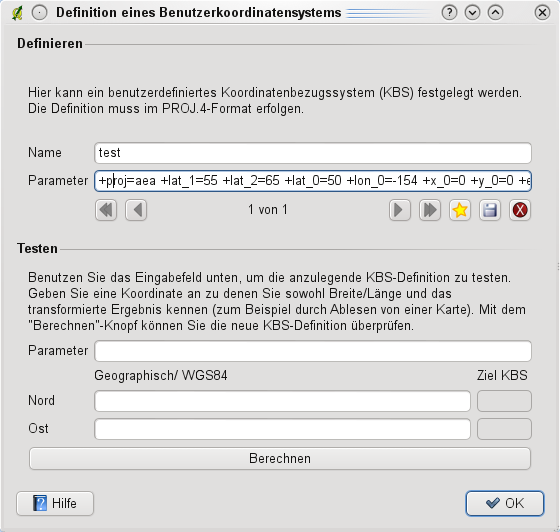
\includegraphics[clip=true, width=8cm]{customProjectionDialog}
   \caption{Диалоговое окно ввода пользовательской проекции
   \wincaption}\label{fig:customprojections}
\end{figure}

Для создания собственной проекции необходимо хорошо разбираться в синтаксисе
библиотеки поддержки картографических проекций PROJ.4. Рекомендуется
ознакомиться с документом <<Cartographic Projection Procedures for
the UNIX Environment "--- A User's Manual>> (Gerald I.~Evenden, U.S.
Geological Survey Open-File Report 90-284, 1990), доступным по адресу
\url{ftp://ftp.remotesensing.org/proj/OF90-284.pdf}.
Данное руководство описывает использование \usertext{proj.4} и связанных
утилит коммандной строки. Картографичские параметры, используемые в
\usertext{proj.4}, описаны в руководстве и совпадают с используемыми в QGIS.

В диалоговом окне \dialog{Определение пользовательской системы координат}
требуется всего два параметра для определения собственной проекции.
\begin{enumerate}
\item имя проекции
\item картографические параметры в формате PROJ.4.
\end{enumerate}
Для создания новой системы координат нажмите кнопку
\toolbtntwo{mIconNew}{Ввод}, укажите имя и введите необходимые параметры. После
чего созданную проекцию можно сохранить путём нажатия кнопки
\toolbtntwo{mActionFileSave}{Сохранить}.

Отметим, что значение поля \guilabel{Параметры} создаваемой проекции должно
начинаться со строки \usertext{+proj=}-block.

Создаваемую проекцию можно проверить.
Для этого вставьте параметры создаваемой проекции в поле
\guilabel{Параметры} раздела \guiheading{Проверка}. Затем введите значения
широты и долготы WGS-84 в поля \guilabel{Север} и \guilabel{Восток}
соответственно. Нажмите кнопку \button{Рассчитать} и сравните результат
с известными значениями вашей проекции.

\FloatBarrier
